\documentclass[french, 12pt]{beamer}

\usepackage[T1]{fontenc}
\usepackage[french]{babel}
\DecimalMathComma
\usepackage{braket}
\usepackage{svg}
% \setsvg{inkscape = '/etc/profiles/per-user/fluteur/bin/inkscape' -z -D}

\usepackage{amsmath}
\usepackage{pgfplots}
\usepackage{amsfonts}
\usepackage{xfrac}
\newcommand{\somme}{\displaystyle\sum}

\usetheme[compress]{Berlin} % {Boadilla}
\beamertemplatenavigationsymbolsempty
\setbeamertemplate{page number in head/foot}[framenumber]
\setbeamertemplate{frametitle}{}
\useoutertheme{split}

\title{Autour des diagrammes de décision quantiques}
\author{Malo Leroy}
\institute{Parcours recherche -- CentraleSupélec}

\usepackage{tikz}
\usetikzlibrary{positioning}
\usepackage{tikz-cd}

\begin{document}

\begin{frame}
    \titlepage
\end{frame}

% 1. Replacez votre projet dans son contexte : enjeux scientifiques, enjeux sociétaux et/ou économiques (le cas échéant)
\begin{frame}{Contexte}

\begin{center}
Les besoins en puissance de calcul croissent rapidement
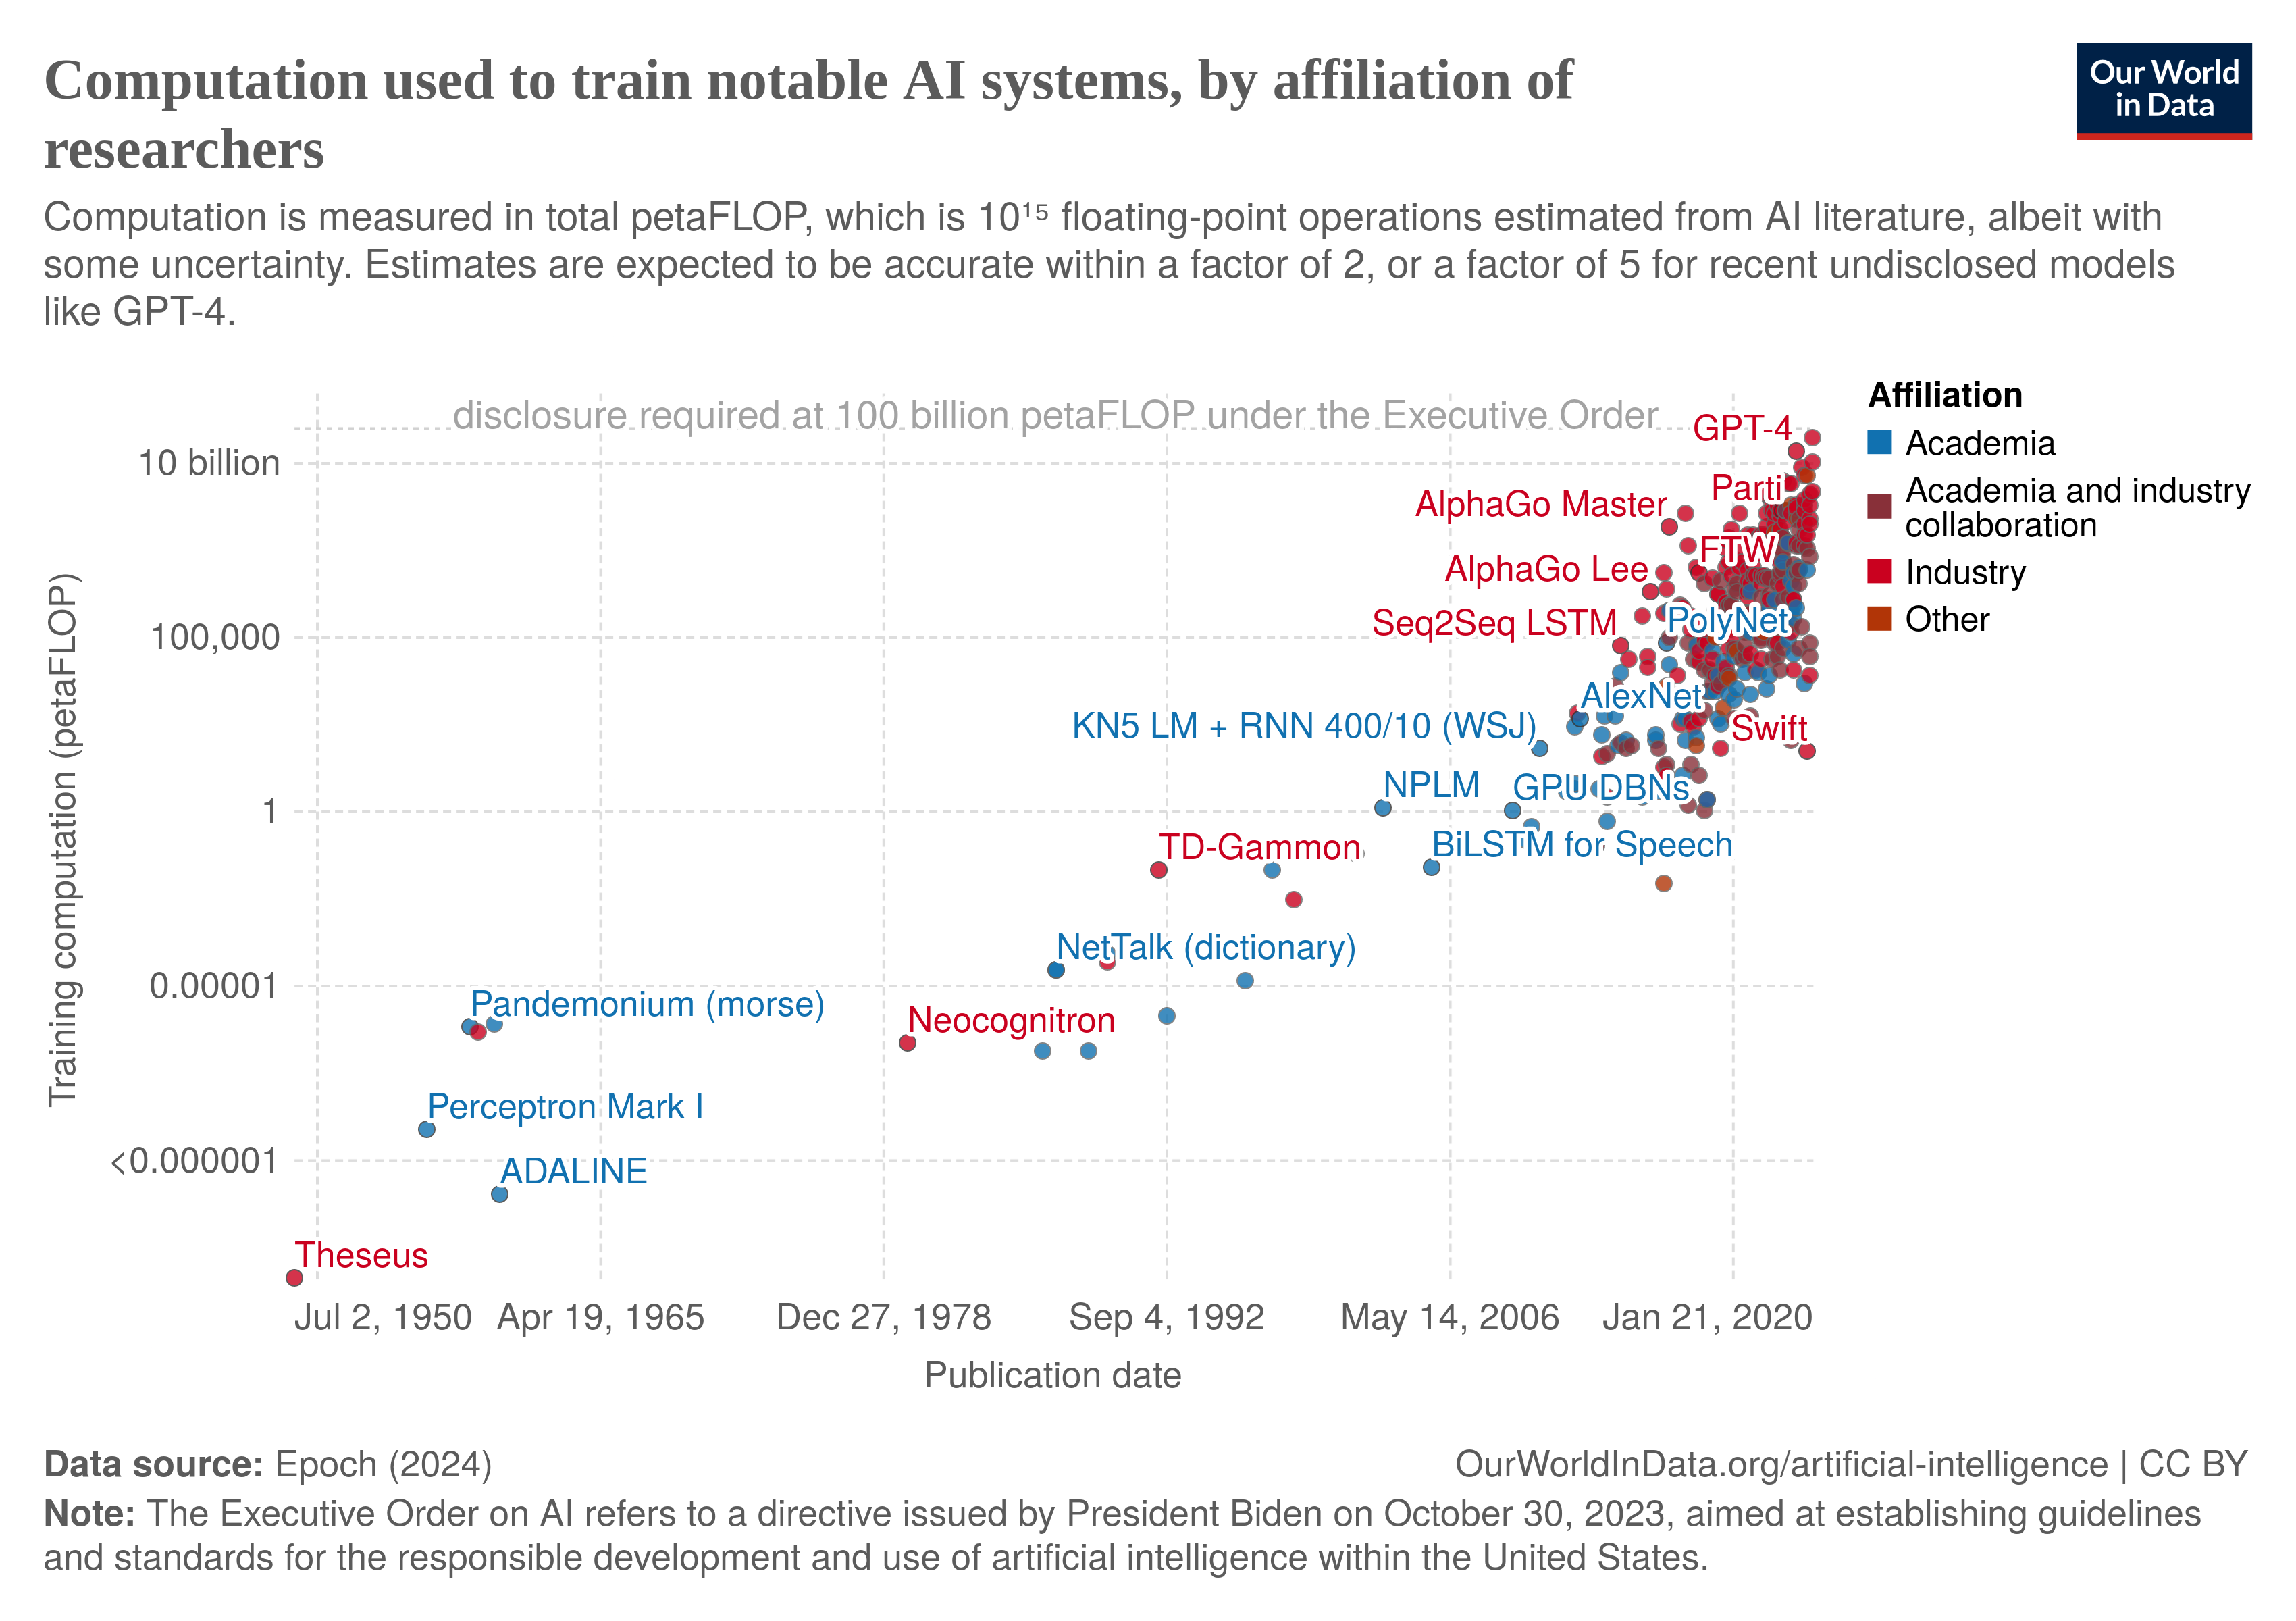
\includegraphics[width=0.6\textwidth]{./images/artificial-intelligence-training-computation-by-researcher-affiliation.png}

Les algorithmes classiques sont parfois inefficaces

\pause
Les \textbf{algorithmes quantiques} permettent de résoudre certains problèmes plus efficacement
\end{center}
\end{frame}

\begin{frame}
Il y a un besoin d'outils de développement et vérification d'algorithmes quantiques
\end{frame}

% état de l'art (ce qui a été déjà fait par d'autres)
\begin{frame}{État de l'art}
\textbf{État de l'art:}
\begin{itemize}
    \item Diagrammes de décision quantiques
    \item Interprétation abstraite
    \item Arithmétique des intervalles réels
\end{itemize}
\pause
\begin{center}
    Solution : \underline{diagrammes additifs abstraits}
\end{center}
\end{frame}

% 2. Présentez les objectifs de votre projet.
\begin{frame}{Objectifs}
Objectifs
\begin{itemize}
    \item \textbf{Modèle formel} de diagrammes de décision additifs abstraits
    \item \textbf{Implémentation} du modèle
\end{itemize}

\end{frame}

% 4. Développez la méthodologie que vous avez mise en œuvre durant ces premiers mois, en la justifiant.
\begin{frame}{Méthodologie de travail}
\underline{\textbf{Méthodologie}}
\small{
\begin{center}
% https://tikzcd.yichuanshen.de/#N4Igdg9gJgpgziAXAbVABwnAlgFyxMJZABgBpiBdUkANwEMAbAVxiRBAF9T1Nd9CUARnJVajFmwA6knDAAeOYABEIAYyYBbGGBx08BDp24gM2fQOQBmEdXrNWiENNkLgAUTkwNaBvENceM34iACZSENE7CUdneUUAFQALAEuIACcsGH9jUz4CIgAWcMjxBycZOOAASW8GZK0dPX5-URgoAHN4IlAAMzSIDSQyEBwIJGExeyQwJgYGagY6ACMYBgAFXnM2Xx6cI17+wcQJ0aQwyejyl0VVOjgAAiY4FgY4QwXl1Y2g-McdvYCID6A3G1FOiGsFzKsVcyV0OHusHuDAA5HQ0jh3iBFit1ptgo4Mu1EgDjMCjudwZCotCKq4NNAABe+LE4r7434gIkkkDUFZgKBISzEQHkoVgsaIIpQqR0m7QLK87GfPE-ATYmC7fZAw7ikaS8406azebK3HfPLq-5K-mCiEism6xCUyXSo0xOXAWRwHBvJVs1WW7aagEUDhAA
\begin{tikzcd}[ampersand replacement=\&, column sep=small]
    {} \arrow[r] \& \text{Documentation} \arrow[rr, "\text{cas usuels}"] \arrow[rdd, "\text{état de l'art}"'] \&                                                                 \& \text{Exemples} \arrow[ldd, "\text{modèle}"', bend left] \arrow[rdd, "\text{tests}"] \&                       \\
                 \&                                                                                           \&                                                                 \&                                                                                      \&                       \\
                 \&                                                                                           \& \text{Théorie} \arrow[rr, "\text{code}"] \arrow[ruu, bend left] \&                                                                                      \& \text{Code}
    \end{tikzcd}
\end{center}
}
\end{frame}

% 5. Présentez votre travail et vos éventuels résultats.
\begin{frame}{Travail réalisé}
\textbf{Modèle}
\begin{itemize}
    \item[\checkmark] Intervalles de $\mathbb C$ cartésiens \& polaires
    \item[\checkmark] Diagrammes
    \item[\checkmark] Approximation locale, globale
    \item[\checkmark] Fusion forcée
    \item[\checkmark] Algorithmes de réduction
\end{itemize}
\end{frame}

\begin{frame}{Travail réalisé}
    \textbf{Implémentation}
    \begin{itemize}
        \item[\checkmark] Intervalles de $\mathbb C$ cartésiens \& polaires
        \item[\checkmark] Diagrammes : construction, évaluation
        \item[\checkmark] Diagrammes aléatoires
        \item[\checkmark] Fusion forcée
        \item[$\sim$] Algorithmes de réduction
    \end{itemize}
\end{frame}

\begin{frame}{Résultats}
    \begin{columns}
        \begin{column}{0.6\textwidth}
            \begin{tikzpicture}[scale=0.8]
                \begin{axis}[grid=both,
                            xmin=0,ymin=0,
                          xmax=5, ymax=10,
                          axis lines=middle,
                          ]
                \addplot[blue]  {x} node[left]{$y=x$};
                \addplot[red]  {2^x} node[above=-1cm] {$y=2^x$};
                \end{axis}
            \end{tikzpicture}
                \end{column}
        \begin{column}{0.4\textwidth}
            L'avantage en nombre de nœuds est \textbf{exponentiel} pour le \textit{proof of concept}
        \end{column}
    \end{columns}
\end{frame}

% 7. Exposez la suite prévue du projet, en particulier en 2e année.
\begin{frame}{Suite du projet}
\textbf{Suite}
\begin{itemize}
    \item Analyse des résultats
    \item \textbf{Ajustements}
    \begin{itemize}
        \item Fonctions d'erreur
        \item Algorithmes de réduction
    \end{itemize}
    \item Nouveaux concepts
    \begin{itemize}
        \item Multi-valuation
        \item Carte locale inversible
    \end{itemize}
\end{itemize}
\end{frame}

\begin{frame}{Cadre du projet Développements futurs}
    \huge{Cadre du projet \\ Formation future}
\end{frame}

% 3. Présentez le contexte dans lequel vous l'effectuez : éventuellement l'équipe, le laboratoire, les partenaires hors CentraleSupélec, les fonctions des professionnels qui vous entourent.
\begin{frame}{Environnement du projet}
    \begin{columns}
        \begin{column}{0.6\textwidth}
            \begin{itemize}
                \item \textbf{Encadrant} : Renaud Vilmart
                \item \textbf{Équipe} : QuaCS
                \item \textbf{Laboratoire} : Laboratoire Méthodes Formelles
            \end{itemize}
        \end{column}
        \begin{column}{0.4\textwidth}
            \begin{center}
                \includesvg[scale=0.17]{./images/lmf-logo.svg}
                \vspace{0.5cm}
                \includesvg[scale=0.3]{./images/quacs-logo.svg}
            \end{center}
        \end{column}
    \end{columns}
\end{frame}

% 8. Résumez vos choix pour la suite en termes de S8, électifs, international, éventuellement césure
\begin{frame}{Année prochaine}
\begin{center}
    Continuer la formation en \textbf{informatique théorique}
\end{center}
\small{Électifs} % envisagés, choix possibles
\footnotesize{
\begin{itemize}
    \item Génie logiciel orienté objet
    \item Informatique théorique
    \item Calcul haute performance
    \item Modèles et sys. pour la gestion de données
\end{itemize}}
\vspace{1em}
\small{Complément scientifique : métaheuristiques}
\end{frame}

\begin{frame}{Année prochaine}
\textbf{S8} envisagés
\begin{itemize}
    \item Digital Tech Year
    \item S8 à CentraleSupélec
    \begin{itemize}
        \item Continuité du projet
    \end{itemize}
    \item Mobilité internationale
\end{itemize}
\end{frame}

% voire souhaits pour la 3e année
\begin{frame}{Perspectives pour la 3\textsuperscript{e} année}
Dominantes / mentions
\vspace{.5em}
\begin{itemize}
    \item \textbf{Informatique et numérique}
    \begin{itemize}
        \item Sciences du logiciel
        \item Architecture des systèmes informatiques
    \end{itemize}
    \item \textbf{Physique et nanotechnologies}
    \begin{itemize}
        \item Quantum engineering
    \end{itemize}
\end{itemize}
\end{frame}

% 9. Terminez par une conclusion synthétique englobant tous les aspects de votre projet.
\begin{frame}{Conclusion}
\begin{center}
    \huge{Conclusion}
\end{center}
\end{frame}

\begin{frame}{Conclusion}
    \begin{center}
        \huge{Questions}
    \end{center}
\end{frame}

\begin{frame}{Comlément sur les césures}
Complément sur les césures
\begin{itemize}
    \item \textbf{Digital Tech Year}
    \begin{itemize}
        \item Semestre au Paris Digital Lab
        \item Semestre en entreprise à l'international
    \end{itemize}
    \item \textbf{Stage}
    \begin{itemize}
        \item Entreprise
        \item Laboratoire
        \item France ou à international
    \end{itemize}
    \item \textbf{Stage en laboratoire}
    \begin{itemize}
        \item En France ou à l'international
    \end{itemize}
\end{itemize}
\end{frame}

\begin{frame}{Pile technique}
Technologies utilisées
\begin{itemize}
    \item \textbf{Code}
    \begin{itemize}
        \item Langage C++
        \item CMake
        \item GNU C Compiler
    \end{itemize}
    \item \textbf{Versionnage}
    \begin{itemize}
        \item Git
        \item GitHub
    \end{itemize}
    \item \textbf{Tests}
    \begin{itemize}
        \item Google Test
        \item GitHub Actions
    \end{itemize}
    \item \textbf{Documentation} Doxygen
\end{itemize}
\end{frame}

\end{document}
